\section{tasks::subtractbias Class Reference}
\label{classtasks_1_1subtractbias}\index{tasks::subtractbias@{tasks::subtractbias}}
Inheritance diagram for tasks::subtractbias::\begin{figure}[H]
\begin{center}
\leavevmode
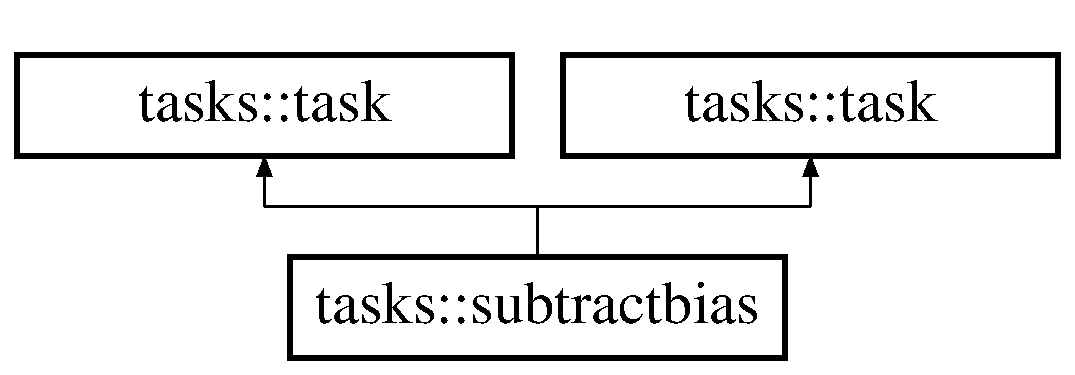
\includegraphics[height=2cm]{classtasks_1_1subtractbias}
\end{center}
\end{figure}
\subsection*{Public Member Functions}
\begin{CompactItemize}
\item 
def \textbf{run}\label{classtasks_1_1subtractbias_8951b67080e7f7a8c7e1275afc658315}

\item 
def \textbf{run}\label{classtasks_1_1subtractbias_8951b67080e7f7a8c7e1275afc658315}

\end{CompactItemize}
\subsection*{Static Public Attributes}
\begin{CompactItemize}
\item 
string \textbf{name} = '{\bfsubtractbias}'\label{classtasks_1_1subtractbias_b75ea77bfcaf6f463a717377a91b0cdf}

\item 
string \textbf{button\-Text} = 'Subtract BIAS'\label{classtasks_1_1subtractbias_7d7fd01b986c11fbcee71be4b9709bbb}

\item 
string \textbf{suffix} = 'bias'\label{classtasks_1_1subtractbias_561eb2a376e8a0b9947c15a9d2431141}

\item 
list \textbf{prereq} = ['{\bfpreproc}']\label{classtasks_1_1subtractbias_ed4f4bc20c3c9fe02bc9a3a2a7762c4a}

\end{CompactItemize}


\subsection{Detailed Description}


\footnotesize\begin{verbatim}Subtract combined BIAS from image.
\end{verbatim}
\normalsize
 



The documentation for this class was generated from the following files:\begin{CompactItemize}
\item 
old/PANICtool-1.0/tasks.py\item 
old/tasks.py\end{CompactItemize}
